\chapter{Kinect}
\label{sec:kinect}

% O Kinect, mostrado na Figura \ref{kinect}, é o nome de um projeto da Microsoft para seu console de videogame Xbox 360, que tem ainda como colaboradora a empresa Prime Sense. O projeto visa criar uma nova tecnologia capaz de permitir aos jogadores interagir com os jogos eletrônicos sem a necessidade de ter em mãos um controle(\textit{joystick}), inovando no campo da jogabilidade.

O \textit{Kinect}, mostrado na Figura~\ref{kinect}, é o nome do acessório desenvolvido pela Microsoft com a colaboração da Prime Sense para seu console de videogame Xbox 360. Tal acessório permite aos jogadores interagir com os jogos eletrônicos sem a necessidade de interagir diretamente com um controle (\textit{joystick}). Devido a este fato o \textit{Kinect} foi considerado uma grande inovação no campo da jogabilidade.

	\begin{figure}[hbt]
		\begin{center}
		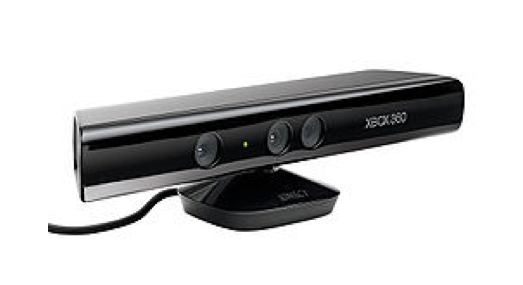
\includegraphics[scale=0.07]{figuras/Apendice/kinect.JPG}
		\end{center}
		\caption{Sensor Kinect da Microsoft.}
		\label{kinect}
	\end{figure}

	A Microsoft define o \textit{Kinect} como ``jogos sem necessidade de controle e experiência de entretenimento''. Porém, seu uso e inovação não se limita apenas no campo dos jogos eletricos (15).

	O \textit{Kinect} possui as seguintes especificações técnicas:

	\begin{itemize}
		\item Sensor
			\begin{itemize}
				\item Lentes com detecção de cores e profundidade
				\item Microfone de voz
				\item Motor de inclinação para ajuste do sensor
			\end{itemize}
		\item Campo de visão
			\begin{itemize}
				\item Campo de visão horizontal: 57 graus
				\item Campo de visão vertical: 43 graus
				\item Alcance físico da inclinação: (+/-) 27 graus
				\item Um alcance máximo de aproximadamente $\displaystyle 4.5$ metros para câmera de profundidade. 
			\end{itemize}
		\item Fluxo de Dados
			\begin{itemize}
				\item 320x240 16-bit depth a 30FPS
				\item 640x480 32-bit color a 30FPS
				\item 16-bit áudio a 16 kHz
			\end{itemize}
	\end{itemize}

Seu hardware é composto por câmeras que obtém imagens de cor, som e que utiliza iluminação infra-vermelha (IR) para obter dados de profundidade~\cite{kinect}. A Figura \ref{kinect_interno} apresenta a organização interna do \textit{Kinect} em alto nível.

	\begin{figure}[hbt]
		\begin{center}
			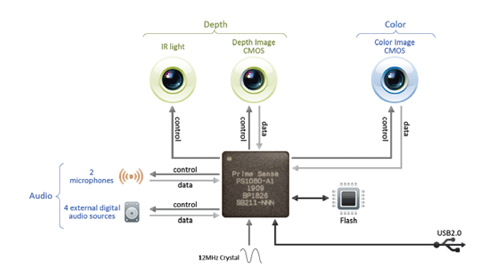
\includegraphics[scale=0.8]{figuras/2.FundamentacaoTeorica/kinect_interno.png}
		\end{center}
		\caption{Organização interna do Kinect~\cite{kinect}.}
		\label{kinect_interno}
	\end{figure}

Um chip especializado é responsável pelo processamento dos dados fornecidos pela câmera de profundidade correlacionando-os com as imagens de cor. O software interno ao \textit{Kinect} combina cada pixel com sua profundidade, processa os dados e os envia a máquina por meio de uma interface USB na forma de mapas de profundidades e imagens de cor~\cite{kinect}.

